% ======================= Pre-Amble =========================

\documentclass[11pt, oneside]{article}   	% use "amsart" instead of "article" for AMSLaTeX format 
                     						%imports package {article} and specify option(s) [11pt, oneside]
\usepackage{geometry}                		% See geometry.pdf to learn the layout options. There are lots.                                        

\geometry{letterpaper}                   		% ... or a4paper or a5paper or ... 
%\geometry{landscape}                		% Activate for rotated page geometry

\usepackage[parfill]{parskip}    		        % Activate to begin paragraphs with an empty line rather than an indent

\usepackage[hidelinks]{hyperref}                % Allows for clickable references

%American Mathematics Society packages
\usepackage{amsmath}	   %math
\usepackage{amssymb}       %symbols
\usepackage{amsthm}          %theorems

%Graphics
\usepackage{graphicx}
\usepackage[usenames, dvipsnames]{color}     % font colour:    \textcolor{<colour>}{text}
      									%highlight text:  \colorbox{<color>}{text}
\usepackage{soul}						%highlight text: \hl     %only  yellow			
									
									%list of colours: https://www.sharelatex.com/learn/Using_colours_in_LaTeX

%Images		                
\graphicspath{ {images/} }                          %directory that your images are located in within your current directory
	

%Footnote Spacing
\setlength{\footnotesep}{0.4cm}                  %specify spacing b/w footnotes
\setlength{\skip\footins}{0.6cm}                    % space b/w footnotes and textbody

%Table
\usepackage[none]{hyphenat}                    % Stops breaking-up words in a table (i.e. no hyphens)
                                                               

\usepackage{array}   
\newcolumntype{x}[1]{>{\centering\let\newline\\\arraybackslash\hspace{0pt}}p{#1}}       %center fixed column width: x{<len>}                      
\newcolumntype{$}{>{\global\let\currentrowstyle\relax}}                                                   % let us apply things (e.g. bold/italicize) to entire row            
\newcolumntype{^}{>{\currentrowstyle}}
\newcommand{\rowstyle}[1]{\gdef\currentrowstyle{#1} #1\ignorespaces}

%Bibliography
\usepackage[numbers,sort&compress]{natbib}   %for multiple references: sorts  (i.e. [1,2] NOT [2, 1] )
                                           				  %                                     compresses (i.e. [1-3] )
\usepackage[nottoc]{tocbibind}                            %add bibliography to table of contents

%Diagrams
\usepackage[latin1]{inputenc}
\usepackage{tikz}
\usetikzlibrary{shapes,arrows,backgrounds}
	

\usepackage{dirtytalk}    %quotations: use \say{}  

\usepackage{caption}
\captionsetup[figure]{labelfont=bf}    %make figure labels boldface
\captionsetup[table]{labelfont=bf}     %make table labels boldface

\usepackage{pgfplots}       %graph in cartesian

%Bullets
\usepackage{enumerate}     %specify type of enumeration: \being{enumerate}[<type of enumeration>]

%QED
\newcommand*{\QEDA}{\hfill\ensuremath{\blacksquare}}         %make qed filled square:    \QEDA
%\newcommand*{\QEDB}{\hfill\ensuremath{\square}}               %make qed empty square: \QEDB 

%Header and Footer
\usepackage{fancyhdr}
\usepackage{lastpage}      %ensures you can reference LastPage (i.e. Page 2 of 10)


%=========== Header & Footer =========================

\pagestyle{fancy}
\lhead{Stephanie Knill} 		% controls the left corner of the header
\chead{} 					% controls the center of the header
\rhead{} 					% controls the right corner of the header
\lfoot{} 					% controls the left corner of the footer
\cfoot{Page~\thepage\ of \pageref{LastPage}} 				% controls the center of the footer
												%Page~\thepage\  if just want Page x
\rfoot{}			 		% controls the right corner of the footer
\renewcommand{\headrulewidth}{0.4pt}
\renewcommand{\footrulewidth}{0.4pt}

% ======================== Document ======================
\begin{document}


\title{MATH 220 --- Assignment 2 \\
\line(1,0){360} }             %(slope x, y){length of line}

\author{
Stephanie Knill \\
54882113 \\
Due: January 12, 2015}

\date{}                   % Activate:  display a given date (e.g. {August 4} ) or no date (empty {} )
                                    %No activate: display current date
\maketitle

\thispagestyle{empty}                   %Remove header from this (first) page. Change empty -> plain to keep numbering


% ================= Questions ================

\section*{Question 1}

Let $U = \{1,3,5, \ldots , 15\}$ be the universal set, $A = \{1,5,9,13\}$, and $B=\{3,9,15\}$.

\begin{enumerate}[ (a)]           
    \item $A \cup B = \{1, 3, 5, 9, 13, 15\}$
    \item $A \cap B = \{9\}$
    \item $A - B = \{1, 5, 13\}$
    \item $B - A = \{3, 15\}$
    \item $\overline{A} = U - A = \{3, 7, 11, 15\}$
    \item Since $\overline{B} = \{1,5,7,11,13\}$, then $A \cap \overline{B} = \{1,5,13\}$   
\end{enumerate}


\section*{Question 2}

Let $U$ be the universal set and let $A, B$ be two subsets of $U$. Then we can express the following sets as Venn diagrams:

\begin{enumerate}[ (a)]           
    \item $\overline{A \cup B}$

        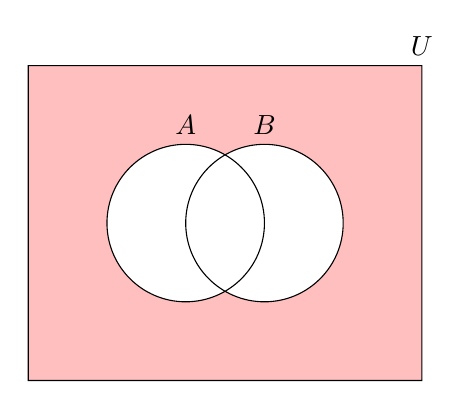
\begin{tikzpicture}[fill=pink]
            % fill rectangle
            \fill (-2,-2) rectangle (3,2);
            
            %fill circles white
            \begin{scope}
                \clip (-2,-2) rectangle (3,2);     %crop location to be filled
                \fill[white] (0,0) circle (1)
               		       (1,0) circle (1);
            \end{scope}
           
            % outline 
            \draw (0,0) circle (1) (0,1)  node [text=black,above] {$A$}      %Draw circle: (center x, center y) circle (radius) 
                      (1,0) circle (1) (1,1)  node [text=black,above] {$B$}      %Label: (label x, label y) [specifiy colour, location]  {label text}
                      (-2,-2) rectangle (3,2) node [text=black,above] {$U$};  %Draw rectangle: (LB x, LB y) rectangle (UB x, UB y); LB & UB on diagonal from each other
        \end{tikzpicture}

%        \begin{tikzpicture}[fill=pink]
%            % fill left hand
%            \begin{scope}
%                \clip (-2,-2) rectangle (2,2)     %crop location to be filled
%                       (1,0) circle (1);
%                \fill (0,0) circle (1);
%            \end{scope}
%            
%            % fill right hand
%            \begin{scope}
%                \clip (-2,-2) rectangle (2,2)
%                        (0,0) circle (1);
%                \fill (1,0) circle (1);
%            \end{scope}
%           
%            % outline 
%            \draw (0,0) circle (1) (0,1)  node [text=black,above] {$A$}      %Draw circle: (center x, center y) circle (radius) 
%                      (1,0) circle (1) (1,1)  node [text=black,above] {$B$}      %Label: (label x, label y) [specifiy colour, location]  {label text}
%                      (-2,-2) rectangle (3,2) node [text=black,above] {$U$};  %Draw rectangle: (LB x, LB y) rectangle (UB x, UB y); LB & UB on diagonal from each other
%        \end{tikzpicture}
            
    
    
    
    \item $\overline{A} \cap \overline{B}$ 
    
    Since $\overline{A \cup B} = \overline{A} \cap \overline{B}$, the Venn Diagram is identical to that in part a).
    
              
    \item $\overline{A \cap B}$
    
            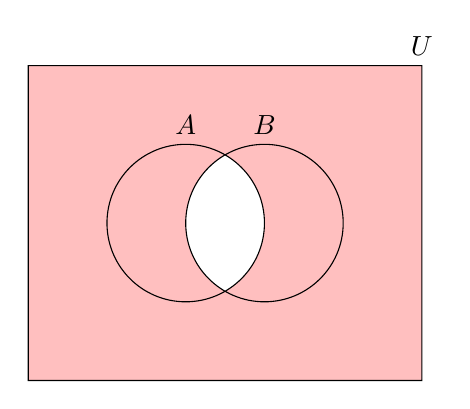
\begin{tikzpicture}[fill=pink]
            % fill rectangle
            \fill (-2,-2) rectangle (3,2);
            
            %fill overlap white
            \begin{scope}
                \clip (1,0) circle (1);
                \fill[white] (0,0) circle (1);
            \end{scope}
           
            % outline 
            \draw (0,0) circle (1) (0,1)  node [text=black,above] {$A$}      %Draw circle: (center x, center y) circle (radius) 
                      (1,0) circle (1) (1,1)  node [text=black,above] {$B$}      %Label: (label x, label y) [specifiy colour, location]  {label text}
                      (-2,-2) rectangle (3,2) node [text=black,above] {$U$};  %Draw rectangle: (LB x, LB y) rectangle (UB x, UB y); LB & UB on diagonal from each other
        \end{tikzpicture}    
    
    \item $\overline{A} \cup \overline{B}$
    
    Since $\overline{A \cap B} = \overline{A} \cup \overline{B}$, the Venn Diagram is identical to that in part c).        
        
\end{enumerate}



\section*{Question 3}

The power set of \{1,2,3\} is given by
$$\mathcal{P}(\{1,2,3\}) = \{ \emptyset, \{1\}, \{2\}, \{3\}, \{1, 2\}, \{1, 3\}, \{2, 3\}, \{1, 2, 3\} \}$$

Looking at the possible permutations for the subsets $A$ and $B$, we can immediately discard any set of subsets where $A = B$ or when one of the subsets is the empty set. Through some experimentation, we find that all eight set operations are unique if $|A| = |B| = 1$. Without loss of generality, let $A=\{1\}$ and $B=\{2\}$.

While we may be tempted to stop here, upon closer examination of the set operations we can see another pair of subsets $C$ and $D$. Let $C = \overline{A}$ and $D = \overline{B}$. Then the set operation $A \cup B$ can be rewritten as $\overline{A} \cup \overline{B}$, the set operation $A \cup \overline{B}$ as $\overline{A} \cup B$, and so forth. Thus, we are simply swapping the order of the conditions for the sets $A$ and $B$. The values for the subset pair $A = \{1\}$ and $B = \{2\}$ and the subset pair $\overline{A} = \{2, 3\}$ and $\overline{B} = \{1,3\}$ are given in Table~\ref{set operations}.

\begin{table}[h]                                          %optional argument: place figure/table here (h), top (t), page of floats (p)
\begin{center}
\begin{tabular}{c | c | c}
    
    & $A = \{1\}$, $B = \{2\}$ & $\overline{A} = \{2, 3\}$, $\overline{B} = \{1,3\}$ \\
    \hline
    $A \cup B$ & $\{1,2\}$ & $\{1,2,3\}$ \\
    $A \cup \overline{B}$ & $\{1,3\}$ & $\{2,3\}$ \\
    $\overline{A} \cup B$ & $\{2,3\}$ & $\{1,3\}$ \\
    $\overline{A} \cup \overline{B}$ & $\{1,2,3\}$ & $\{1,2\}$ \\
    \hline
    $A \cap B$ & $\emptyset$ & $\{3\}$ \\
    $A \cap \overline{B}$ & $\{1\}$ & $\{2\}$ \\
    $\overline{A} \cap B$ & $\{2\}$ & $\{1\}$ \\
    $\overline{A} \cap \overline{B}$ & $\{3\}$ & $\emptyset$ \\

\end{tabular}
\end{center}
\caption{Set operations performed on $A$ and $B$, and $\overline{A}$ and $\overline{B}$.}
\label{set operations}
\end{table}


\section*{Question 4}

For a real number $r$, define $S_r$ to be the interval $[r-1, r+2]$. Let $A=\{1,3,4\}$. Then
\begin{align*}
\bigcup_{\alpha \in A} S_{\alpha} & = S_1 \cup S_3 \cup S_4 \\
& = [(1)-1, (1)+2] \cup [(3)-1, (3)+2] \cup [(4)-1, (4)+2] \\
& = [0, 3] \cup [2,5] \cup [3,6] \\
& =[0,6]
\end{align*}

and

\begin{align*}
\bigcap_{\alpha \in A} S_{\alpha} & = S_1 \cap S_3 \cap S_4 \\
& = [(1)-1, (1)+2] \cap [(3)-1, (3)+2] \cap [(4)-1, (4)+2] \\
& = [0, 3] \cap [2,5] \cap [3,6] \\
& =[3]
\end{align*}

\section*{Question 5}

Let $A_n = \{n, n-1\}$ for every $n \in \mathbb{N}$. Then

\begin{align*}
\bigcup_{n \in \mathbb{N}} A_n & = \{1,0\} \cup \{2,1\} \cup \{3,2\} \cup \dots \\
& = \{0\} \cup \mathbb{N}
\end{align*}

and

\begin{align*}
\bigcap_{n \in \mathbb{N}} A_n &  = \{1,0\} \cap \{2,1\} \cap \{3,2\} \cap \dots \\
& = \emptyset
\end{align*}


\section*{Question 6}

For $A=\{1,2\}$ and $B=\{1\}$, the cartesian product $A \times B$ is given by
$$A \times B = \{(1, 1), (2, 1)\}$$

Thus we can compute the power set of $A \times B$ to be 
$$\mathcal{P}(A \times B) = \{\emptyset, \{(1,1)\}, \{(2,1)\}, \{(1,1), (2,1)\}\,\}$$


\section*{Question 7}

For $A = \{a \in \mathbb{R} : |a| \leq 1\}$ and $B = \{b \in \mathbb{R} : |b| = 1\}$, we can geometrically describe the points in the $xy$-plane belonging to $(A \times B) \cup (B \times A)$ as the disk $C$ of radius 1 centered at the origin in the $xy$-plane. In other words, $x^2 + y^2 \leq 1$, where $x,y \in \mathbb{R}^2$.

%\begin{center}
%\begin{tikzpicture}
%
%    \begin{axis}[axis lines=middle,axis equal,grid=both]
%    \addplot coordinates{(-3,1) (6,-2)};				%line: \addplot coordinates{(-3,1) (6,-2)};
%    \end{axis}
%
%\end{tikzpicture}
%\end{center}


\end{document} 